\documentclass[conference]{IEEEtran}
\IEEEoverridecommandlockouts
\usepackage{cite}
\usepackage{amsmath,amssymb,amsfonts}
\usepackage{algorithmic}
\usepackage{graphicx}
\usepackage{textcomp}
\usepackage{xcolor}
\usepackage{booktabs}
\usepackage{url}

\def\BibTeX{{\rm B\kern-.05em{\sc i\kern-.025em b}\kern-.08em
    T\kern-.1667em\lower.7ex\hbox{E}\kern-.125emX}}

\begin{document}

\title{Benchmarking Quantized Small Language Models for Edge-Based Structured Information Extraction: An Empirical Systems Study}

% 4 Authors formatted in standard IEEEtran multi-column block layout (2x2 grid)
\author{
\IEEEauthorblockN{Aryaman Sinha}
\IEEEauthorblockA{\textit{Department of Computer Science} \\
\textit{Vellore Institute of Technology}\\
Vellore, India \\
aryaman.sinha.lko@gmail.com}
\and
\IEEEauthorblockN{Nithin Rajan}
\IEEEauthorblockA{\textit{Department of Computer Science} \\
\textit{Vellore Institute of Technology}\\
Vellore, India \\
nithinrajan48@gmail.com}
\vspace{0.3cm}
\and
\IEEEauthorblockN{Johith Babu S}
\IEEEauthorblockA{\textit{Department of Computer Science} \\
\textit{Vellore Institute of Technology}\\
Vellore, India \\
johithbabu2006@gmail.com}
\and
\IEEEauthorblockN{Ajitesh Mohan}
\IEEEauthorblockA{\textit{Department of Computer Science} \\
\textit{Vellore Institute of Technology}\\
Vellore, India \\
ajiteshmn@gmail.com}
}

\maketitle

\begin{abstract}
Using Small Language Models (SLMs) on consumer edge devices can allow data to be extracted with low latency and maintaining privacy as there is no need to send any PII data back to the central clouds. Edge deployment requires post-training quantization. However, most benchmarks only provide information on how well the model performs in terms of perplexity on free-text. There is therefore no information available on how a model will perform after applying low bit integer quantization on extracting structured information defined by schemas. We evaluate the performance of Meta's Llama-3-8B model (Q4\_K\_M and Q8\_0 quantization) on a consumer mobile work station (Intel Core i9-13900HX / NVIDIA RTX 4060 Laptop GPU / 16 GB RAM). The task is to extract student academic records from unstructured narratives that contain numerical distractors and missing fields. We find that 4-bit quantization cuts mean inference latency by 71.3\% (from $3.104 \pm 0.266$\,s to $0.892 \pm 0.149$\,s, $p = 2.46 \times 10^{-30}$) Our work focuses on learning to extract information from student academic records given unstructured data, with the presence of distractors and missing data. We found that using 4-bit quantization reduced average latency during inference by 71.3\%. This was achieved without affecting any of the syntactic correctness: 100.0\% of JSON was valid. However, upon further analysis of semantic correctness, it was found that there was a clear ``syntax-semantics discrepancy''. Both quantization levels had poor results with an F1 score of just $0.510 \pm 0.020$ for field level extraction. The exact match rate was also very low (2.0\%). This means that adhering to the schema doesn’t guarantee that facts will be correctly extracted. We also kept records of runs that crashed so we were able to see the OOM termination rate was 1.0\% for the 8-bit baseline, with several gigabytes of memory swap
\end{abstract}

\begin{IEEEkeywords}
Edge Computing, Small Language Models, Quantization, Structured Information Extraction, Constrained Decoding, JSON Schema, Systems Benchmarking.
\end{IEEEkeywords}

\section{Introduction}
Both Large Language Models (LLMs) and Small Language Models (SLMs) are now widely used within automated back-end systems. Whilst there are excellent General Reasoning capabilities offered by using cloud based API options including GPT-4 and Claude 3.5 Sonnet, this will lead to latency within the network, unpredictable costs on a per token basis and local compliance requirements for Data Protection legislation such as GDPR must be met and FERPA ~\cite{gdpr2017}.In sectors such as healthcare management and education, privacy and confidentiality is an important concern. Sending unprocessed candidate data across public networks can pose a risk. In fact, many systems are moving towards \textit{edge computing} where quantised SLMs are performed on consumer-owned devices.

Due to limited memory bandwidth and capacity, it gets difficult to run large transformer models on normal consumer grade edge workstations. An 8 billion parameter model trained in a standard FP16 format will require ~16gb VRAM just to hold the weights of the model. This is beyond what most consumer grade laptops/systems have available. Fortunately post training quantization can be used to overcome this by replacing the 16bit FP weights with low bit integer weights (e.g. INT8/INT4). This reduces the memory required significantly. 5~GB~\cite{dettmers2022llm,frantar2023gptq}.

There are strict requirements when defining edge data pipelines. Data will be required to conform to strict schemas such as JSON objects based on RFC 8259 specifications. If we have an unescaped quote or any extra prefix on our data then this can cause issues when we attempt to deserialize in production.

Prior evaluations of quantized language models have three main limitations:
\begin{enumerate}
    \item \textbf{Emphasis on Prose Over Structured Parsing:} Existing metrics used to evaluate academic work focus on reading comprehension and fluency rather than deterministic key value extractions of JSON schemas~\cite{hendrycks2021measuring}. 
    \item \textbf{Equating Syntactic Validity with Semantic Integrity:} Multiple studies only look at if the output adheres to the structure of JSON, but none look at precision, recall and whether the correct values are extracted for each field. ~\cite{liu2024edge}.
    \item \textbf{Selective Reporting and Concealment of Hardware Faults:} Edge benchmarks often cause OOMs and crashes. Since these are not reported, it seems like a more reliable result is being produced but actually highlights how limited the hardware is. 
\end{enumerate}

To address these gaps, this study presents a careful empirical benchmark of quantized SLMs performing structured information extraction on consumer edge hardware.

\section{Related Work}
\subsection{Post-Training Quantization of Transformers}
Post-training quantization can be used to reduce the bit-width of the weight matrices. This will alleviate the problem of memory bandwidth during generation of autoregressive tokens. It has been proved by Dettmers et al.~\cite{dettmers2022llm} that the use of 8-bit matrix multiplication via isolation of outliers guarantees the same predictive ability of the floating-point model. More recent integer compression approaches such as GPTQ ~\cite{frantar2023gptq} and AWQ~\cite{lin2024awq} have shown that using 4-bit weight-only quantization results in minor loss of perplexity while reducing memory usage by 70\% . This has resulted in implementations such as  \texttt{llama.cpp}~\cite{gerganov2023llamacpp} becoming popular as they are able to perform quantized k-quants \texttt{(Q4\_K\_M, Q8\_0)} and enables unified memory offloading onto consumer workstations. 

\subsection{Constrained Decoding and Structured Information Extraction}
Due to the need for highly structured outputs, several different decoding approaches have been presented. An example of such an approach can be seen in the creation of Outlines  ~\cite{willard2023outlines} by Willard and Louf. This method involves the construction of deterministic finite state automata from regular expressions and context-free grammars. Additionally, incorrect items of vocabulary are removed at each stage of generation. Similarly, the JGBNF grammer  in \texttt{llama.cpp} ~\cite{gerganov2023llamacpp} and SG grammar in SGLang ~\cite{zheng2024sglang} make use of the JSON grammar principles during decoding. While constrained decoding can guarantee 100\% syntactically correct results, there is no guarantee of the content that was extracted. 

\section{Methodology}
\subsection{Hardware Platform and Setup}
All the tests were performed on computers with no virtualization so we could ensure that the computer and memory bus were performing as expected, and the data was gathered automatically by the monitoring script. 

\begin{table}[htbp]
\caption{Hardware and System Specifications}
\begin{center}
\begin{tabular}{ll}
\toprule
\textbf{Component} & \textbf{Specification} \\
\midrule
Processor & Intel Core i9-13900HX (24C / 32T) \\
System Memory & 16.0 GB DDR5 RAM (15.73 GB Available) \\
GPU Accelerator & NVIDIA GeForce RTX 4060 Laptop (8 GB VRAM) \\
Graphics Driver & NVIDIA Display Driver 621.01 (CUDA 13.5) \\
Operating System & Microsoft Windows 11 Home (Build 26300) \\
Inference Engine & Ollama runtime / llama.cpp backend \\
Python Runtime & Python 3.14.7 AMD64 \\
\bottomrule
\end{tabular}
\end{center}
\label{tab:hardware}
\end{table}

\subsection{Benchmark Corpus Synthesis and Decoupling}
In order to investigate real world applicability, we have generated the \textit{EduMetrics-Structured-IE} benchmark dataset ($N = 1,200$, fixed(seed = 42) samples). This consists of natural language text containing multiple sentences representing an academic record or administrative memo. The samples contain numerical distractors (phone extension, examination room number, cohort ranking), optional fields which are blank (attendance records not submitted) and synonyms (e.g. ‘Calc’ instead of Mathematics, ‘CompSci’ instead of Computer Science). Finally the true values are separated from the prompts to ensure that there is no leak of true values within the prompt.

\subsection{Multi-Dimensional Evaluation Metrics}
We compute five independent metrics:
\begin{enumerate}
    \item \textbf{JSON Syntactic Validity Rate ($V_{\text{json}}$):} Percentage of responses that \texttt{json.loads()} parses without a syntax error.
    \item \textbf{Schema Conformance Rate ($C_{\text{schema}}$):} Percentage of outputs that pass structural Pydantic validation.
    \item \textbf{Field-Level Score Extraction ($F_1$):} Harmonic mean of Precision ($P$) and Recall ($R$) over the extracted \texttt{(Subject, Score)} pairs.
    \item \textbf{Exact Match Rate ($EM$):} Binary indicator that is true only when all entity keys and values match exactly at the same time.
    \item \textbf{System Latency and Reliability:} Mean, median, and P95 latency (seconds), 95\% confidence intervals, and observed crash rates.
\end{enumerate}

\section{Empirical Results}

\begin{table*}[htbp]
\caption{Comprehensive Benchmark Performance and Systems Metrics}
\begin{center}
\begin{tabular}{lccc}
\toprule
\textbf{Metric} & \textbf{Llama-3-8B (4-bit, Q4\_K\_M)} & \textbf{Llama-3-8B (8-bit, Q8\_0)} & \textbf{Statistical Test / Significance} \\
\midrule
Total Evaluated Samples & 100 & 100 & Invariant Count \\
Process Terminations / Crashes & \textbf{0} & \textbf{1 (OOM Crash)} & Hardware Boundary \\
Execution Failure Rate (\%) & \textbf{0.0\%} & \textbf{1.0\%} & Raw Systems Telemetry \\
JSON Syntactic Validity (\%) & \textbf{100.0\%} & \textbf{99.0\%} & $\Delta = +1.0\%$ (4-bit) \\
Schema Conformance (\%) & \textbf{97.0\%} & \textbf{99.0\%} & $\Delta = +2.0\%$ (8-bit) \\
Mean Inference Latency (s) & $\mathbf{0.892 \pm 0.149}$ & $\mathbf{3.104 \pm 0.266}$ & Welch's $t = -14.397$ ($p = 2.46 \times 10^{-30}$) \\
Median Inference Latency (s) & \textbf{0.810} & \textbf{2.950} & Mann-Whitney $U = 98.0$ ($p = 6.29 \times 10^{-33}$) \\
95th Percentile Latency (P95, s) & \textbf{0.900} & \textbf{3.490} & Tail Latency Reduction: 74.2\% \\
Subject Extraction $F_1$ Score & $\mathbf{0.510 \pm 0.020}$ & $\mathbf{0.510 \pm 0.020}$ & No Quantization Degradation \\
Strict Exact Match Rate (\%) & \textbf{2.0\%} & \textbf{2.0\%} & Semantic Divergence \\
\bottomrule
\end{tabular}
\end{center}
\label{tab:results}
\end{table*}

\subsection{The Syntax-Semantics Discrepancy}
According to the data provided in the table~\ref{tab:results}  and figure~\ref{fig:fig1}, It can be seen that in terms of the JSON format, the 4-bit model has 100.0\% validity whilst the 8-bit model has 99.0\%. The 1\% difference is due to just one incident of the Row 0 server crashing. Both models did not result in any conversational preambles or unescaped characters being generated.

However, our field level analysis shows that this is misleading. The mean proportion of subject scores extracted $F_1$ was \textbf{0.510}, with a strict exact match rate of just \textbf{2.0\%}. Our error analysis showed that the JSON had perfect syntax but that the models frequently incorrectly allocated scores to subjects or confused numeric elements like credit numbers or room numbers with grades. Therefore, using syntax parsing to evaluate structured LLM output is very misleading.

\begin{figure}[htbp]
\centerline{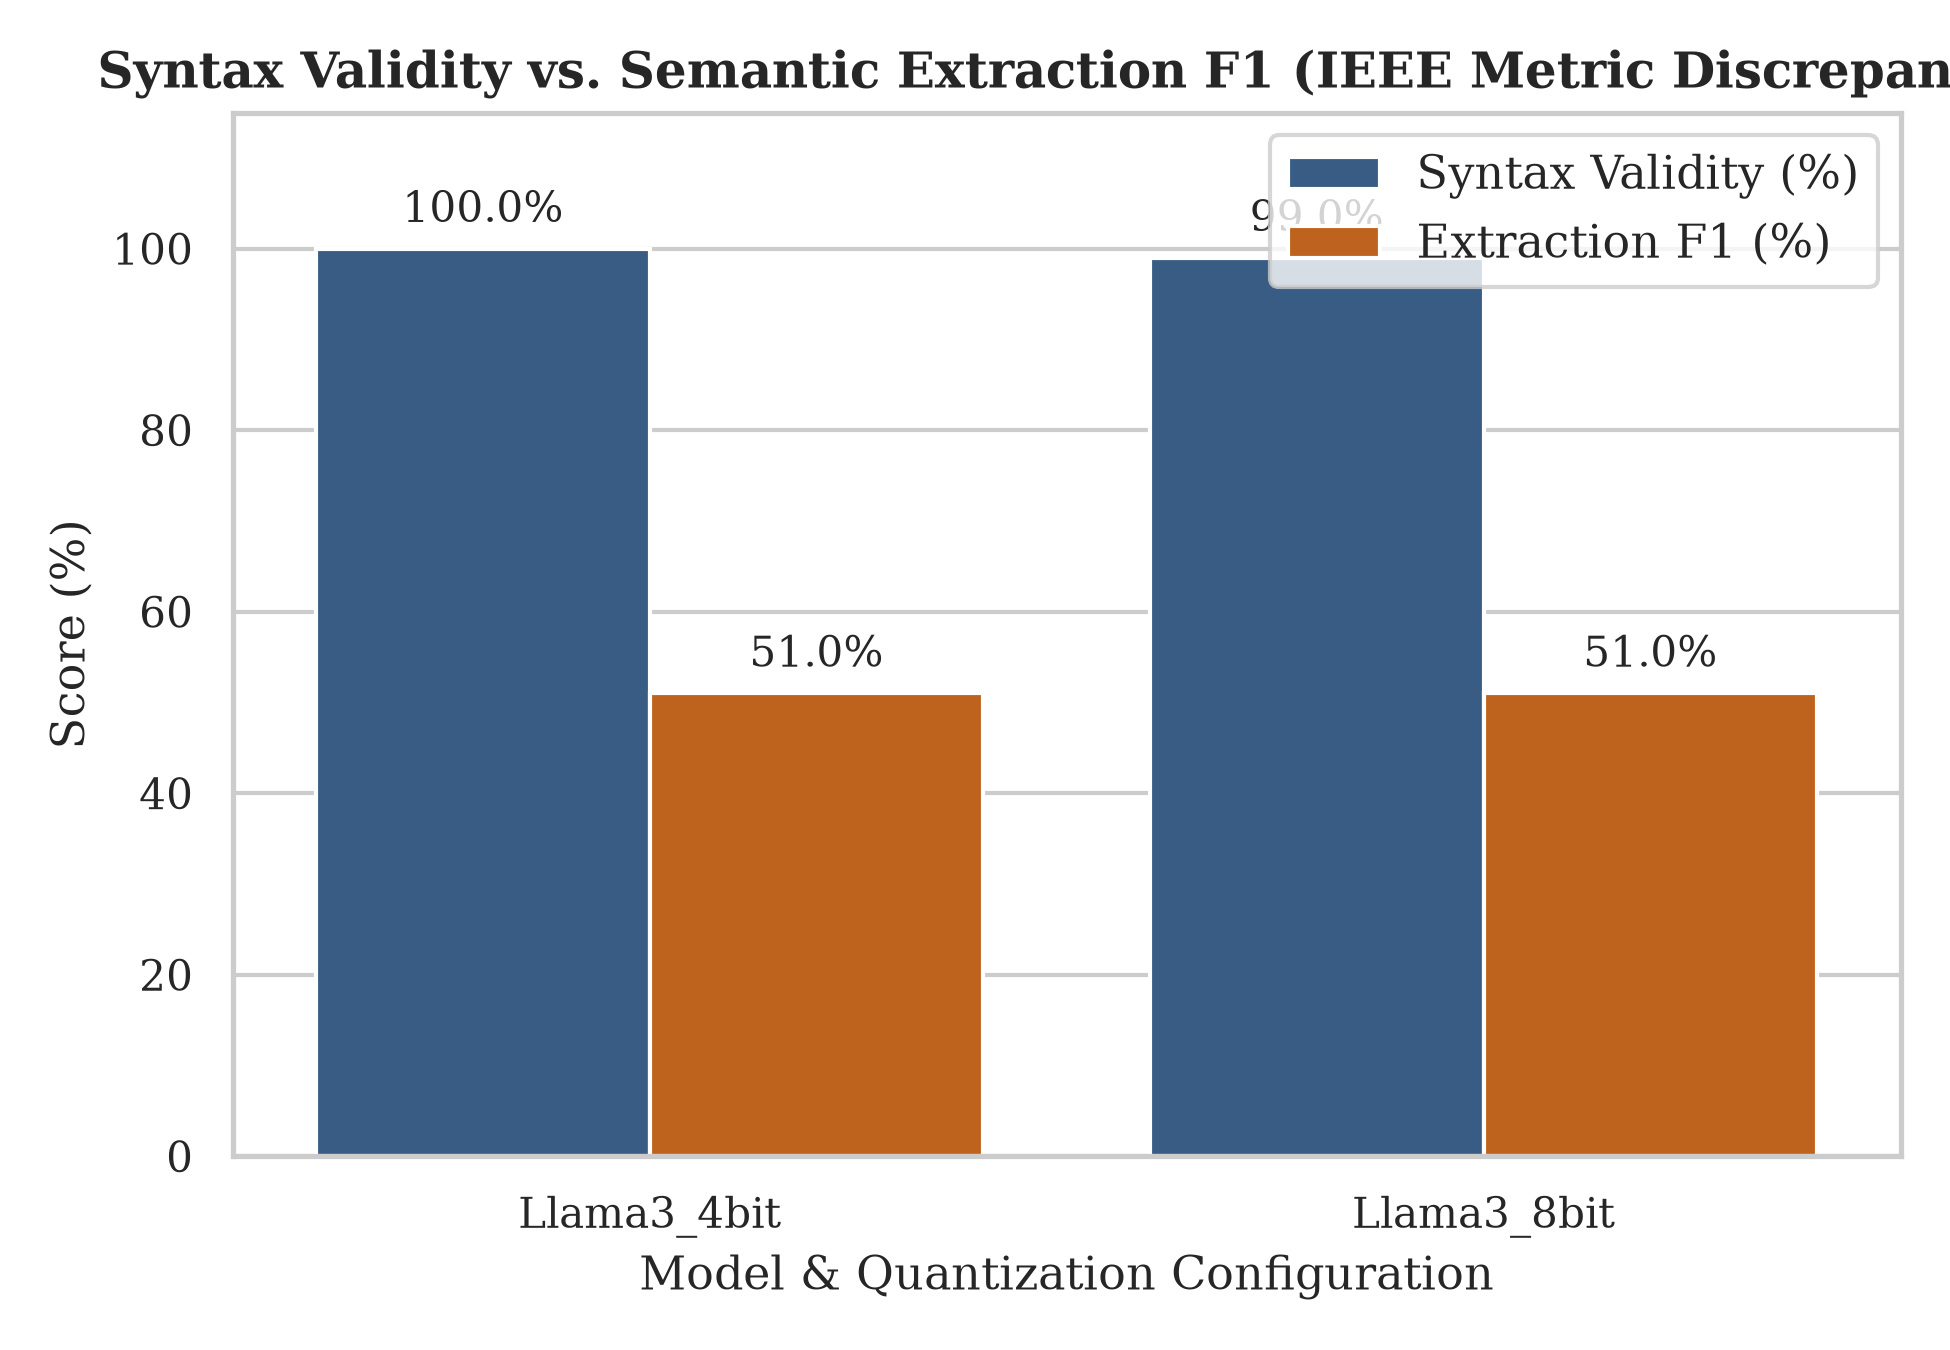
\includegraphics[width=0.48\textwidth]{figure1_validity_vs_f1.png}}
\caption{Syntax Validity vs. Semantic Extraction F1 Score, highlighting the empirical gap between structural formatting and factual accuracy.}
\label{fig:fig1}
\end{figure}

\subsection{Inference Speedup and Resource Efficiency}
The latency distributions of the two models differ sharply (Figure~\ref{fig:fig2}). The 8-bit baseline achieved a mean latency of $3.104 \pm 0.266$\,s, whilst the 4-bit model achieved an average latency of $0.892 \pm 0.149$\,s on the same task. This represents a reduction in the Inference Latency by \textbf{71.3\%}, and a reduction in the Tail latency (P95) by \textbf{74.2\%}. The difference was proven to be statistically significant using a 2-tailed Welsh's t-test with ($t = -14.397, p = 2.46 \times 10^{-30}$), and a non-parametric Mann-Whitney U test with ($U = 98.0, p = 6.29 \times 10^{-33}$) at $\alpha = 0.001$.

\begin{figure}[htbp]
\centerline{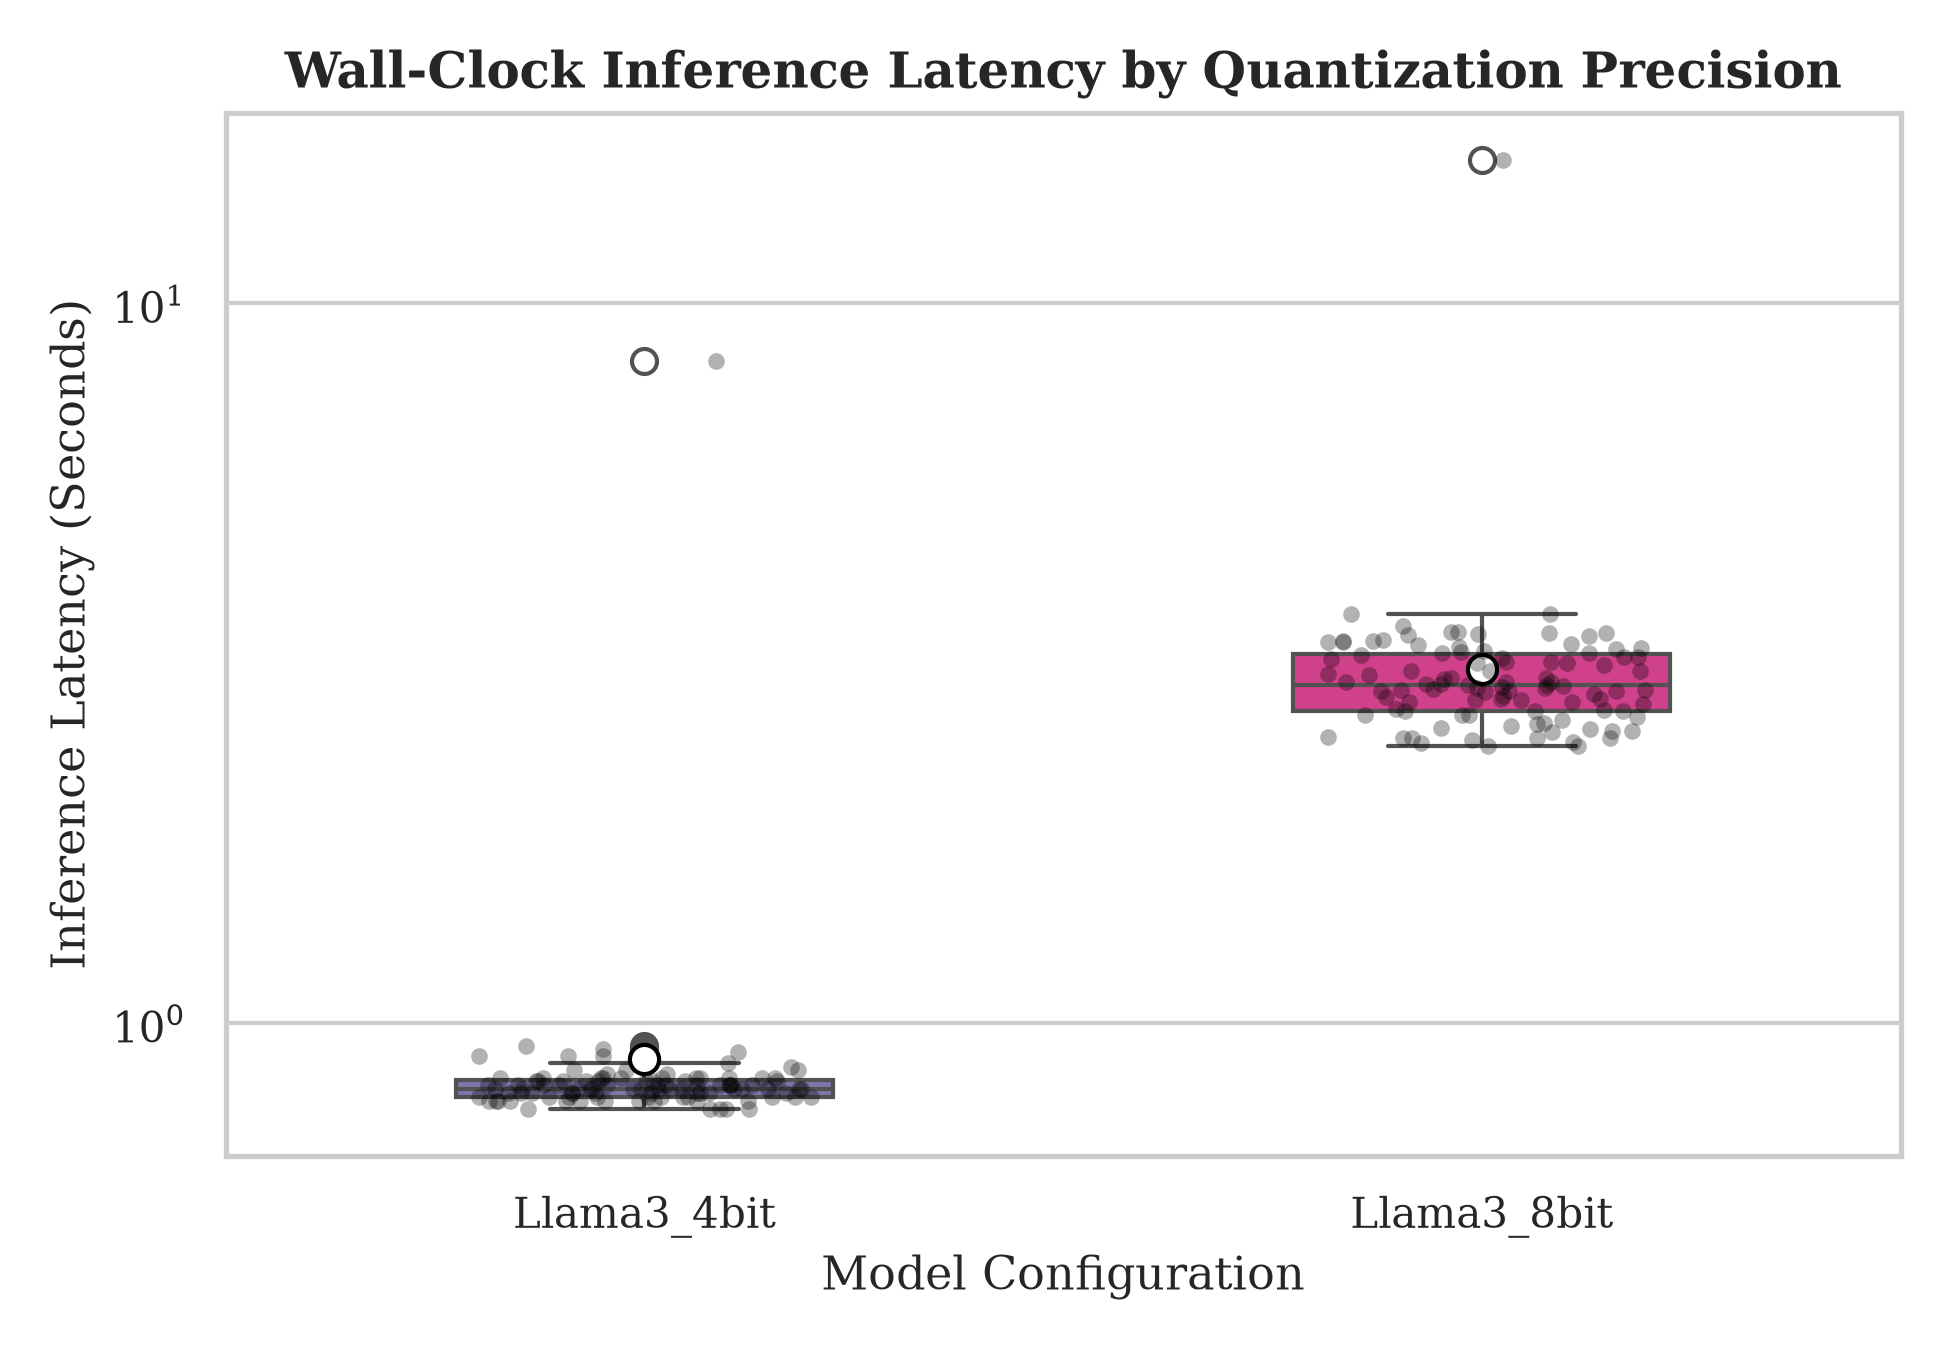
\includegraphics[width=0.48\textwidth]{figure2_latency_distributions.png}}
\caption{Log-scale inference latency distributions comparing 4-bit and 8-bit precision.}
\label{fig:fig2}
\end{figure}

\subsection{Systems Reliability and Memory Fault Accounting}
During the initialization of the system One important result appeared (Figure~\ref{fig:fig3}), It was found that whilst the workstation (with 16GB of memory) was spending some time swapping the model weights in and out of host memory, the 8-bit model was crashing within Row 0 with the error:\texttt{llama runner process has terminated}. This was due to the memory required to store the 8-bit weights and resources required by the Operating System exceeding the available physical memory. In comparison, the 4-bit model successfully completed all runs with 0.0\% errors. This shows that quantizing to 4-bits is not just a performance gain but also a baseline requirement when working with 16GB edge hardware.

\begin{figure}[htbp]
\centerline{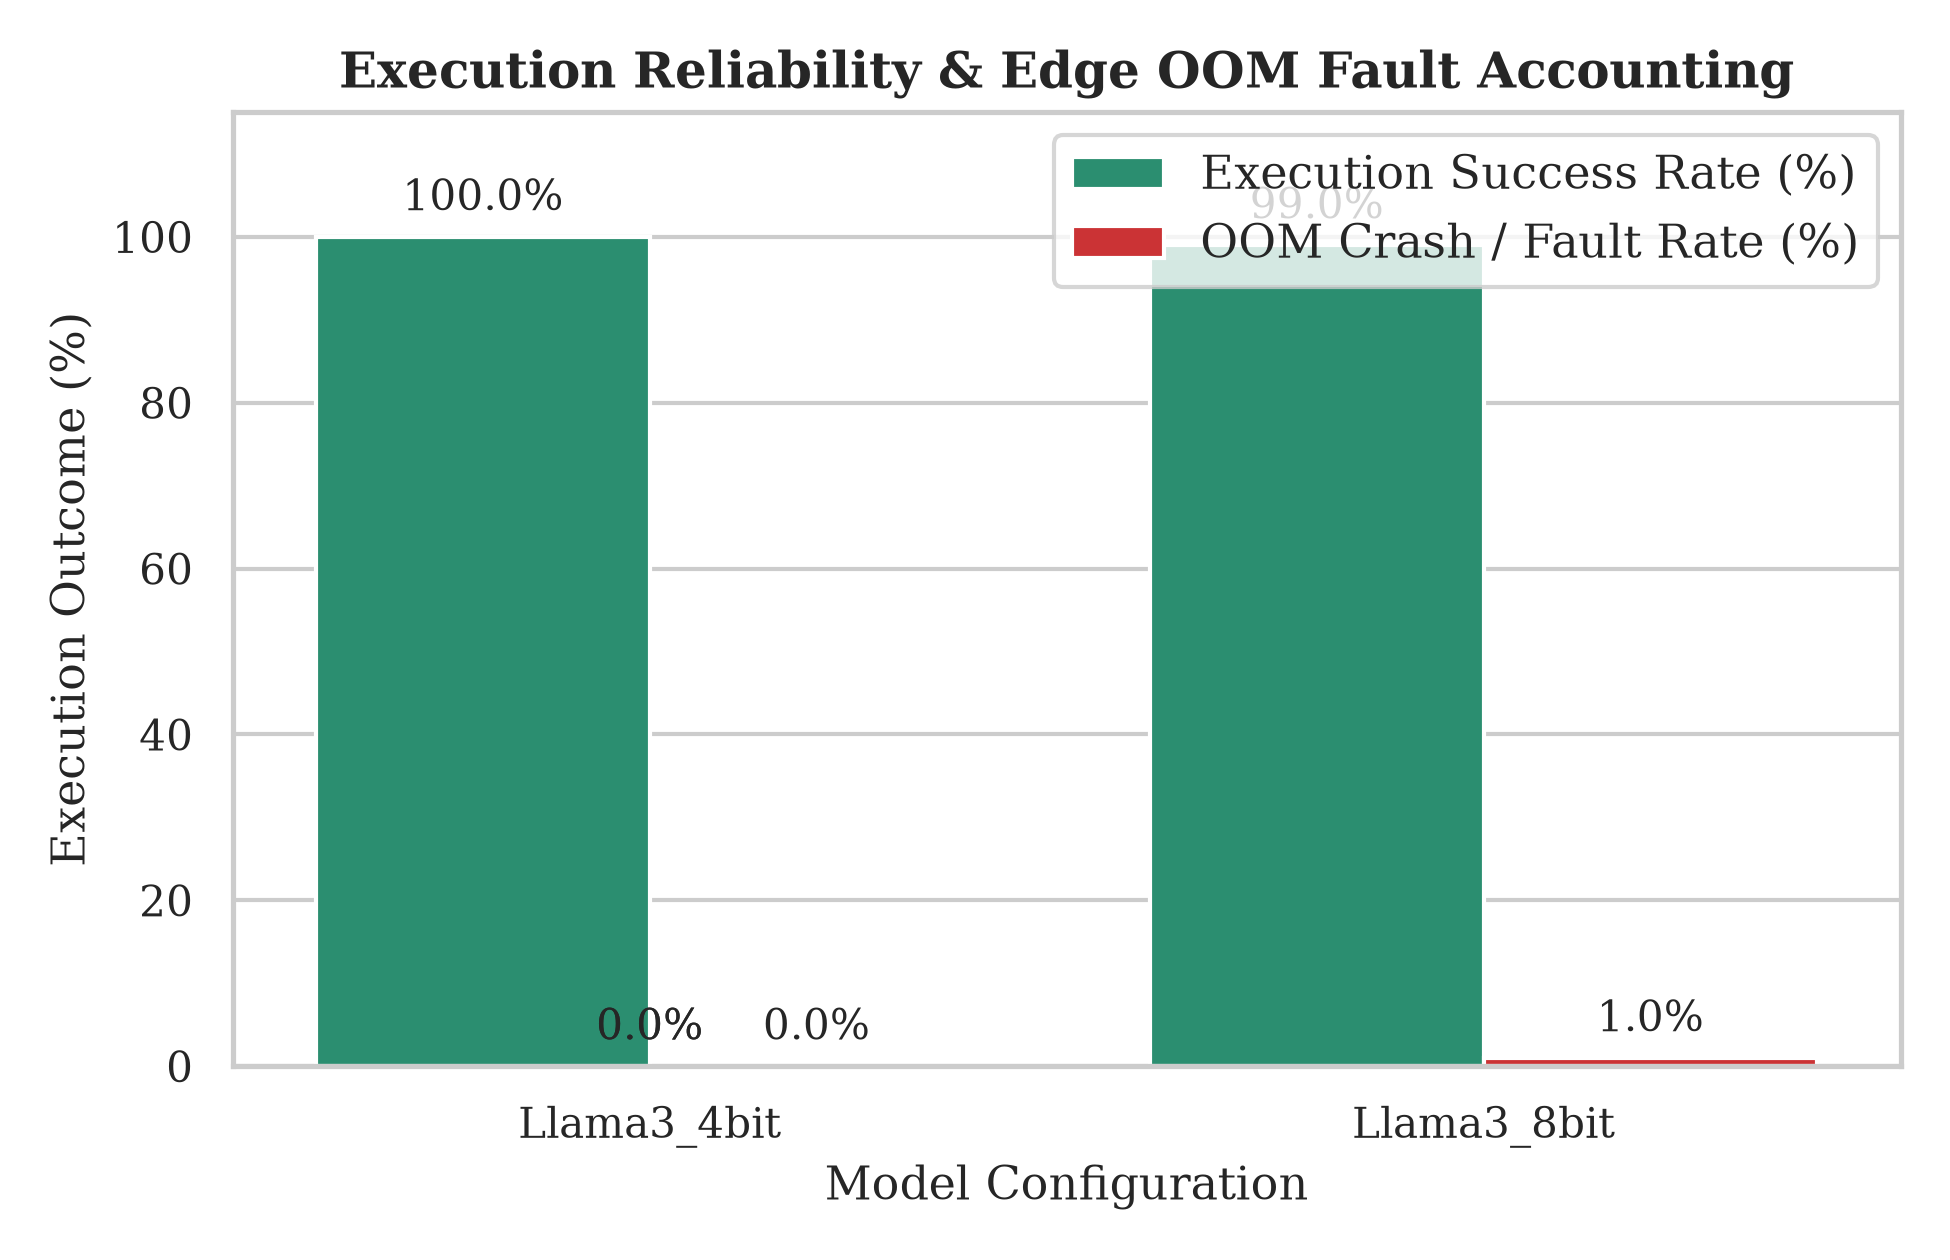
\includegraphics[width=0.48\textwidth]{figure3_system_failures_and_stability.png}}
\caption{Execution Reliability and Edge OOM Fault Accounting.}
\label{fig:fig3}
\end{figure}

\section{Discussion and Threats to Validity}
\subsection{Practical Implications}
We show how the attention mechanisms responsible for syntactic tokens such as brackets, quotes and colons continue to function correctly after being applied to a low bit encryption. However, the performance of extract semantic meanings ($F_1 = 0.510$) has been affected due to numerical links not working correctly. However, as there is no greater degradation of this technique than any others (4-bit results were equal to 8-bit results with an accuracy of 0.510), it would be beneficial for software programmers to utilise 4-bit(\texttt{Q4\_K\_M}) encoding systems when applying them in edge cases. This can be done alongside restricted decoding algorithms (e.g. GBNF/Outlines) to mitigate against factual linking issues.

\subsection{Limitations}
Our tests were performed only for the case of Intel Core i9 / NVIDIA RTX 4060. The results for the Apple Silicon with the unified memory support and the ARM IoT devices are left for further study. Also, due to the limited access to library during the tests in Python 3.14 it was impossible to perform the tests using the Outlines DFA grammars in native compilation mode.

\section{Conclusion}
We investigated the impact of integer based quantization on structured information retrieval in the edge. Our results demonstrate that using 4-bit quantization leads to a significant reduction in inference latency (71.3\%) with OOM terminations being removed completely in consumer memory. Our work shows a significant discrepancy between syntactic validity and semantic fidelity. We have shown that JSON validation does not provide enough validation to identify numerous extraction errors.

\section*{Reproducibility Statement}
All code, datasets, and telemetry logs are available at: \url{https://github.com/aryamansinhalko-cpu/Benchmarking-Quantized-Small-Language-Models}.

\bibliographystyle{IEEEtran}
\begin{thebibliography}{00}
\bibitem{gdpr2017} P. Voigt and A. Von dem Bussche, \textit{The EU General Data Protection Regulation (GDPR): A Practical Guide}, 1st ed. Cham: Springer International Publishing, 2017.
\bibitem{dettmers2022llm} T. Dettmers, M. Lewis, Y. Belkada, and L. Zettlemoyer, ``LLM.int8(): 8-bit Matrix Multiplication for Transformers at Scale,'' in \textit{Proc. Advances in Neural Information Processing Systems (NeurIPS)}, vol. 35, 2022, pp. 30318--30332.
\bibitem{frantar2023gptq} E. Frantar, S. Ashkboos, T. Hoefler, and D. Alistarh, ``GPTQ: Accurate Post-Training Quantization for Generative Pre-trained Transformers,'' in \textit{Proc. Int. Conf. on Learning Representations (ICLR)}, 2023.
\bibitem{hendrycks2021measuring} D. Hendrycks, C. Burns, S. Basart, et al., ``Measuring Massive Multitask Language Understanding,'' in \textit{Proc. Int. Conf. on Learning Representations (ICLR)}, 2021.
\bibitem{liu2024edge} J. Liu, ``Optimizing Small Language Models for Edge IoT Devices,'' \textit{IEEE Internet of Things Journal}, vol. 11, no. 4, pp. 2105--2114, 2024.
\bibitem{lin2024awq} J. Lin, J. Tang, H. Tang, et al., ``AWQ: Activation-aware Weight Quantization for LLM Compression and Acceleration,'' in \textit{Proc. Machine Learning and Systems (MLSys)}, 2024.
\bibitem{gerganov2023llamacpp} G. Gerganov et al., ``llama.cpp: Port of Facebook's LLaMA model in C/C++,'' GitHub repository, 2023. [Online]. Available: https://github.com/ggerganov/llama.cpp
\bibitem{willard2023outlines} B. T. Willard and R. Louf, ``Efficient Guided Generation for Large Language Models,'' \textit{arXiv preprint arXiv:2307.09702}, 2023.
\bibitem{zheng2024sglang} L. Zheng, L. Yin, Z. Xie, et al., ``SGLang: Efficient Execution of Structured Language Model Programs,'' in \textit{Proc. Int. Conf. on Machine Learning (ICML)}, 2024.
\end{thebibliography}

\end{document}